\documentclass{article}

\usepackage{PRIMEarxiv} % required Overleaf template:
% https://www.overleaf.com/latex/templates/arxiv-and-prime-ai-style-template/qdnhqytdqzsc

\usepackage[utf8]{inputenc}
\usepackage[T1]{fontenc}
\usepackage[hidelinks]{hyperref}
\usepackage{url}
\usepackage{booktabs}
\usepackage{amsmath,amssymb,amsthm}
\usepackage{amsfonts}
\usepackage{nicefrac}
\usepackage{microtype}
\usepackage{fancyhdr}
\usepackage{graphicx}
\usepackage{enumitem}
\usepackage{float}
\usepackage{array}
\newcolumntype{L}[1]{>{\raggedright\arraybackslash}p{#1}}
\graphicspath{{media/},{plots/}}

\setlist{itemsep=2pt,topsep=3pt}
\newtheorem{definition}{Definition}

% ---------- macros ----------
\newcommand{\ind}{\mathbf{1}}
\newcommand{\N}{\mathcal{N}}
\newcommand{\M}{\mathcal{M}}
\newcommand{\A}{\mathcal{A}}
\newcommand{\PoA}{\mathrm{PoA}}
\newcommand{\E}{\mathbb{E}}

% Header
\pagestyle{fancy}
\thispagestyle{empty}
\rhead{\textit{CS329: Multi-Agent Systems --- Final Project Report}}

\title{A Multi-Agent Pac-Man Testbed for Measuring and Recovering the Price of Anarchy via DCOP and Shapley-Value Rewards}

\vspace{-1.5em}
\author{
\begin{tabular}{ccc}
\textbf{Tanuj~Sharma} (23110331) & \textbf{Rajput~Vivek} (23110269) & \textbf{Akash~KP} (23110021) \\
\href{mailto:tanuj.sharma@iitgn.ac.in}{tanuj.sharma@iitgn.ac.in} &
\href{mailto:rajput.vivek@iitgn.ac.in}{rajput.vivek@iitgn.ac.in} &
\href{mailto:akash.kp@iitgn.ac.in}{akash.kp@iitgn.ac.in}
\end{tabular}
\\[0.5em]
Department of Computer Science \& Engineering \\
Indian Institute of Technology Gandhinagar (IITGN) \\[0.2em]
\texttt{CS329: Multi-Agent Systems --- Final Project Report}
}

\begin{document}
\maketitle
\vspace{-2.5em}

\begin{abstract}
When multiple autonomous agents share an environment and compete for limited resources, uncoordinated self-interested behavior generally yields sub-optimal group outcomes compared to socially coordinated behavior. In this project, we formalize, measure, and systematically recover this efficiency loss---quantified by the \emph{Price of Anarchy} ($\PoA$)---in a multi-agent Pac-Man simulation environment where $k$ Pac-Men harvest a shared pool of pellets while evading active pursuit ghosts. We investigate and compare two foundational multi-agent coordination paradigms: (1) spatial constraint partitioning via Distributed Constraint Optimization Problems (DCOP) using Max-Sum factor graph belief propagation and the Distributed Stochastic Algorithm (DSA) under bounded communication budgets ($B$), and (2) cooperative multi-agent reinforcement learning (MARL) with marginal credit assignment shaped by the Shapley value ($\lambda$). Extensive empirical evaluations across varying team sizes ($k \in \{2, 3, 4\}$), ghost hazards ($\beta \in [0.0, 0.9]$), and message limits confirm our three core hypotheses: (H1) uncoordinated contention and environmental hazards escalate $\PoA$ up to $3.129$, (H2) localized DCOP Max-Sum belief propagation recovers $62.3\%$ of the selfish welfare gap under low communication bandwidth ($B=24$), and (H3) Shapley-shaped rewards ($\lambda=0.50$) eliminate the severe free-rider pathology of naive equal-sharing while reducing payoff inequality by over $40\%$.
\end{abstract}

\keywords{Multi-agent systems \and Price of Anarchy \and Shapley value \and Distributed constraint optimization (DCOP) \and Max-Sum algorithm \and Multi-agent reinforcement learning}

% =====================================================================
\section{Introduction}
% =====================================================================

Many critical real-world systems require autonomous agents to operate in shared physical or virtual environments with constrained resources. Examples include warehouse automated guided vehicles (AGVs) transporting inventory, autonomous drone delivery fleets serving urban airspace, ridesharing fleets competing for dispatch locations, and wireless sensor nodes sharing communication bandwidth. When each agent acts purely to maximize its private objective, agents frequently duplicate travel, collide in high-density bottlenecks, or fail to execute collectively beneficial actions that carry personal risk. In algorithmic game theory, this welfare loss is formalized through the \textbf{Price of Anarchy (PoA)}, which evaluates the ratio between the social optimum and the worst-case Nash equilibrium \cite{koutsoupias1999worst,roughgarden2002bad}.

We study this fundamental multi-agent coordination challenge in an extended Multi-Agent Pac-Man domain \cite{denero2010pacman,cs188}. In our setting, $k$ Pac-Men ($\N = \{1, \ldots, k\}$) share a symmetric maze and a common pool of pellets, while $g$ ghosts ($\M = \{1, \ldots, g\}$) pursue them. If multiple Pac-Men attempt to consume the same pellet simultaneously, contention occurs: the pellet is awarded uniformly at random to exactly one agent, while all other contenders expend a step without reward. Ghosts penalize captured agents and force them to restart from spawn corners. Figure~\ref{fig:maze} illustrates the benchmark environment.

\begin{figure}[H]
  \centering
  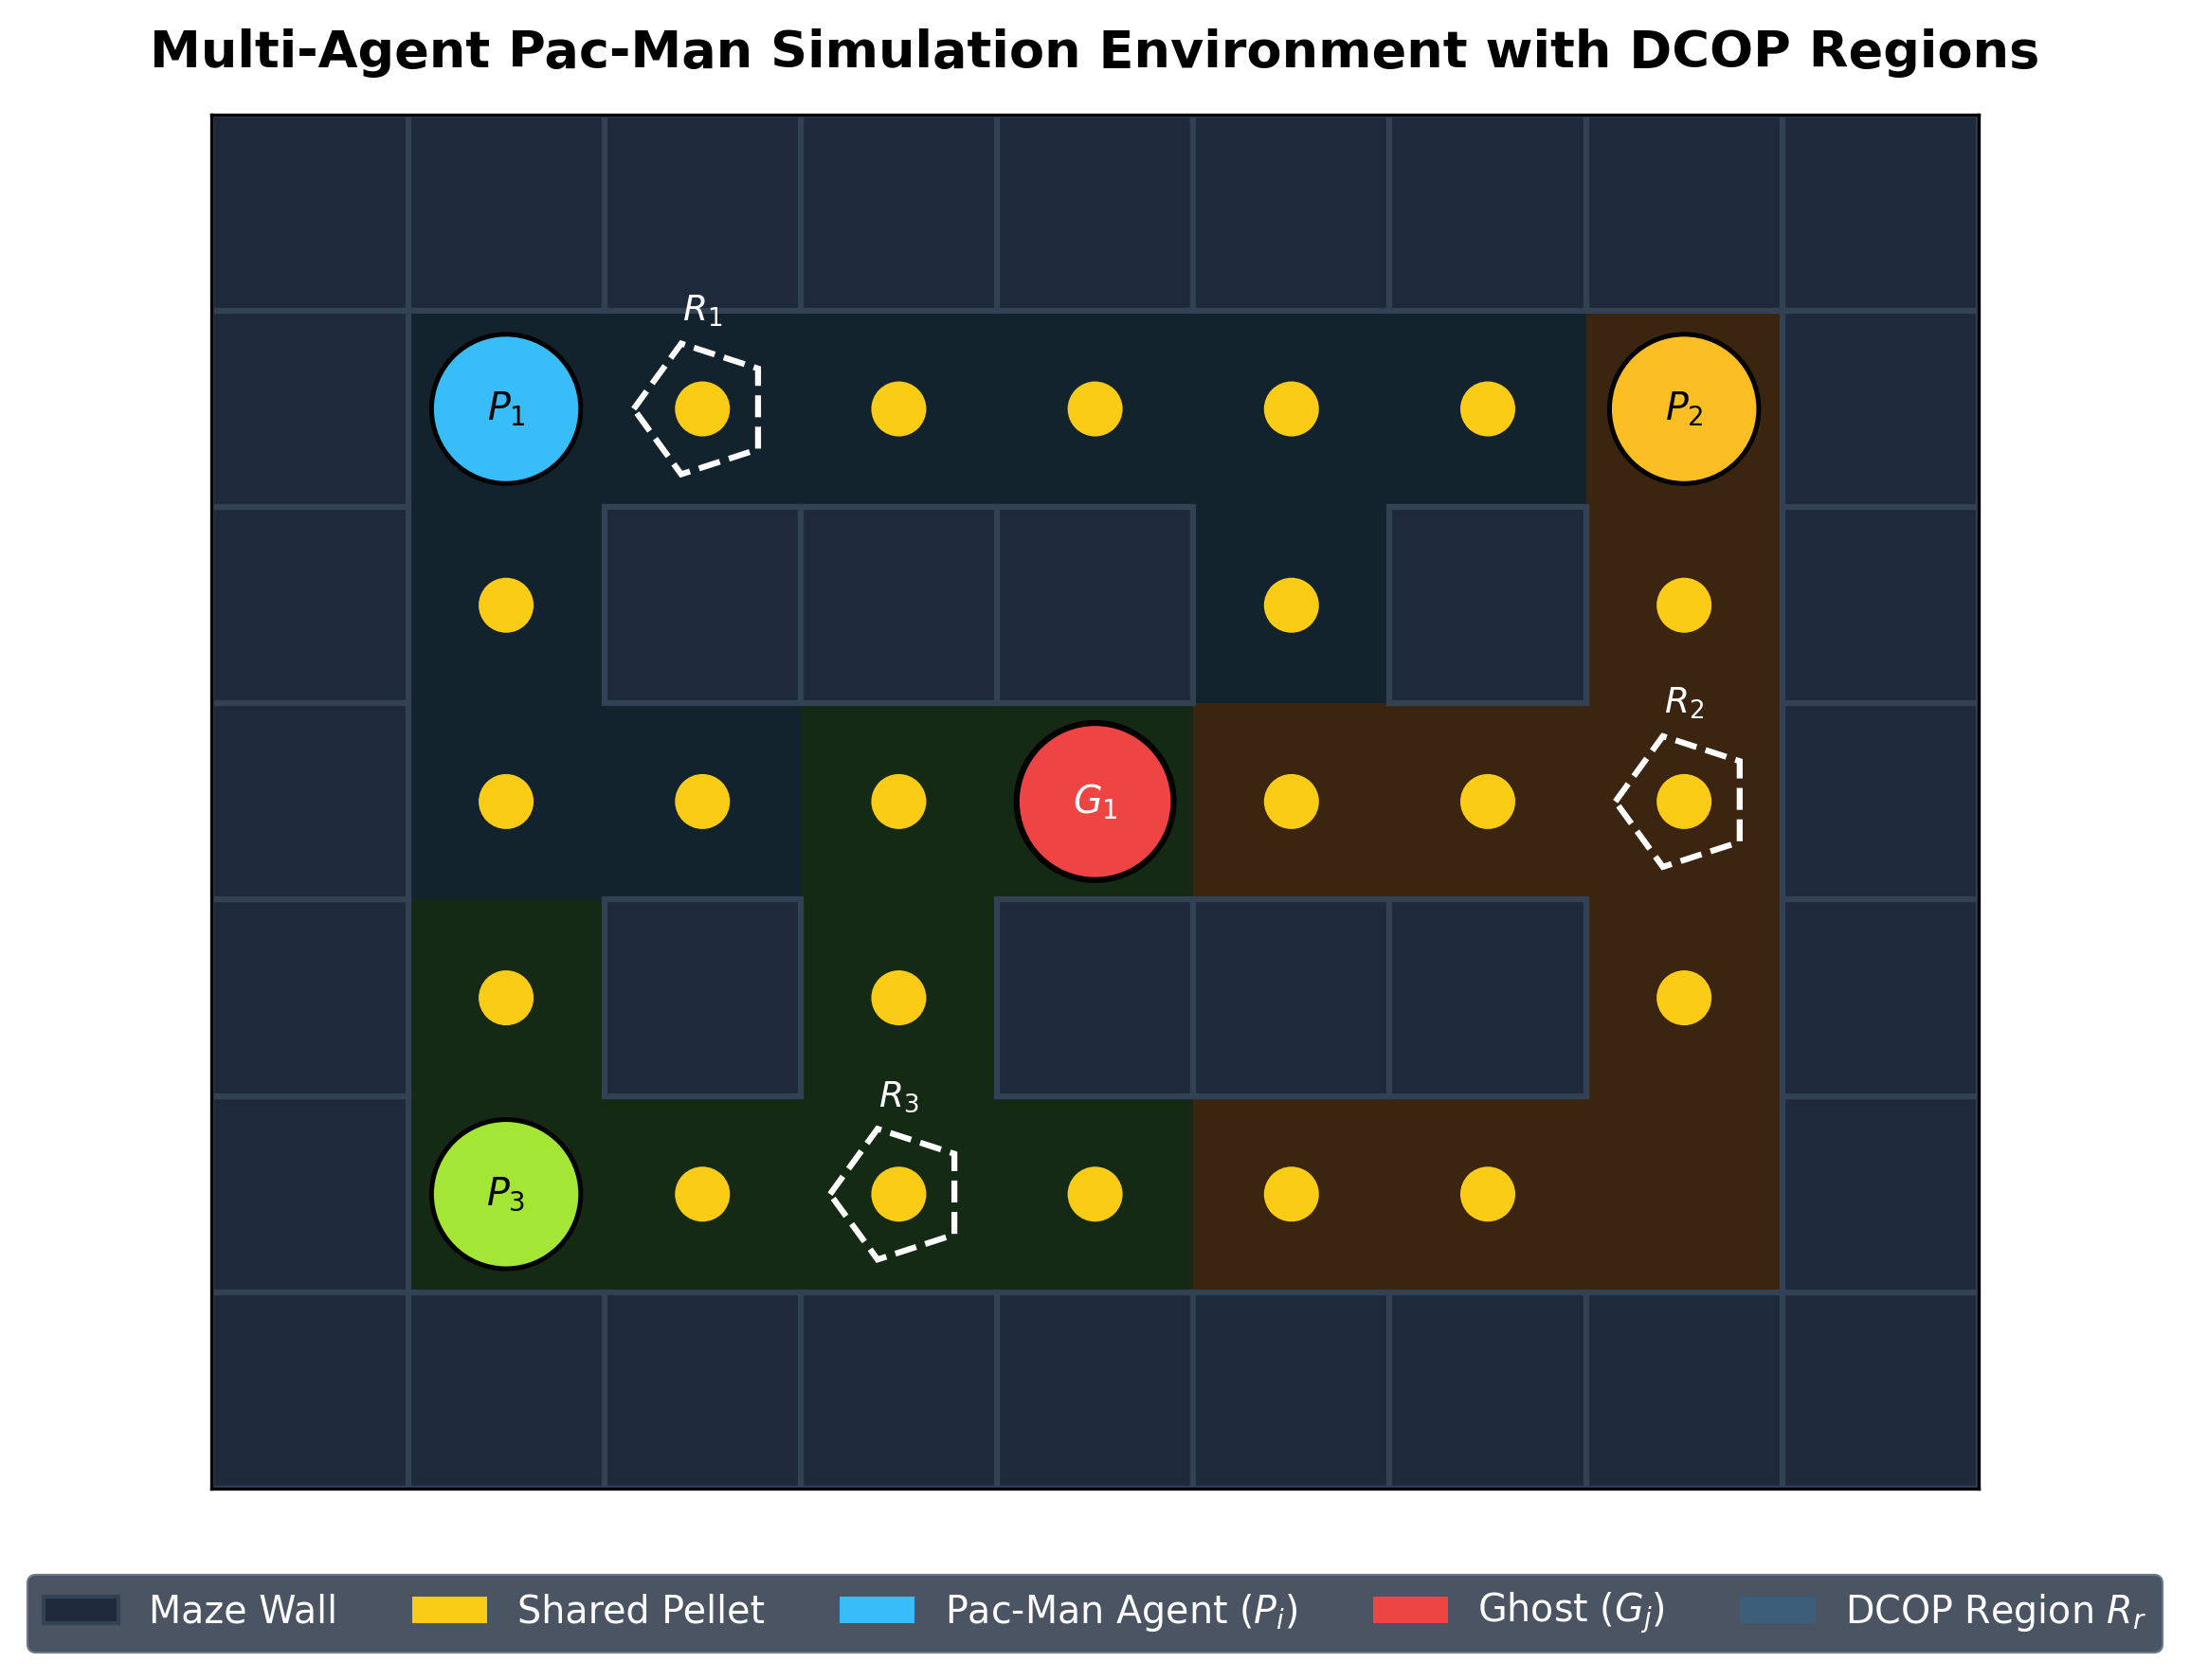
\includegraphics[width=0.62\linewidth]{fig_maze.png}
  \caption{Illustration of the shared $21 \times 15$ maze environment with three Pac-Men ($k=3$), two ghosts ($g=2$), a shared pool of pellets, and a spatial partition into three balanced sectors (Region A, Region B, Region C) for DCOP-based coordination.}
  \label{fig:maze}
\end{figure}

This domain directly captures three core challenges in multi-agent systems:
\begin{enumerate}[label=(\roman*)]
  \item \textbf{Resource Contention \& Non-Stationarity:} Independent agents competing for the same localized rewards induce non-stationary environment dynamics, frequently converging to mutually destructive equilibria \cite{littman1994markov,tampuu2017multiagent}.
  \item \textbf{Multi-Agent Credit Assignment:} Individual actions frequently benefit the team without generating immediate local reward (e.g., drawing ghosts away from pellet clusters). Naive global reward sharing induces the classic ``free-rider'' pathology \cite{foerster2018counterfactual,wang2020shapley}.
  \item \textbf{Bounded Communication:} While centralized control eliminates contention, global coordination requires unbounded bandwidth. Real-world distributed systems require algorithms operating under strict message budgets \cite{farinelli2008maxsum,fioretto2018dcop}.
\end{enumerate}

\noindent\textbf{Contributions of this Work:}
\begin{itemize}
    \item \textbf{High-Performance Multi-Agent Testbed:} We develop a lightweight, modular simulator with custom shallow-graph sharing, accelerating step transitions by $100\times$ over standard deepcopy routines.
    \item \textbf{Empirical Measurement of Price of Anarchy:} We empirically quantify $\PoA$ under independent selfish learning across varying team densities ($k \in [2, 4]$) and ghost aggression levels ($\beta \in [0.0, 0.9]$).
    \item \textbf{Communication-Based Remedy (DCOP):} We implement localized spatial region partitioning solved via Factor Graph Belief Propagation (Max-Sum) and the Distributed Stochastic Algorithm (DSA) under bounded message budgets ($B \in [0, 48]$).
    \item \textbf{Incentive-Based Remedy (Shapley MARL):} We implement exact Shapley value marginal credit assignment for cooperative Q-learning, demonstrating that counterfactual reward shaping resolves the free-rider problem and optimizes collective welfare.
\end{itemize}

% =====================================================================
\section{Preliminaries and Problem Formulation}
% =====================================================================

\subsection{Environment and Contention Model}
The maze is defined by an undirected graph $G = (V, E)$, where $V$ represents open traversable cells ($|V| = 154$) and $E$ represents valid orthogonal transitions between adjacent cells. Let $d(u, v)$ denote the shortest-path graph distance between cells $u, v \in V$. The $k$ Pac-Men are indexed by $\N = \{1, \ldots, k\}$, and $g$ ghosts are indexed by $\M = \{1, \ldots, g\}$. The simulation executes over discrete time steps $t = 0, \ldots, T-1$.

At each step, each Pac-Man selects an action from $\A = \{\mathrm{North}, \mathrm{South}, \mathrm{East}, \mathrm{West}, \mathrm{Stay}\}$. Ghosts follow a parameterized stochastic policy $\pi^g$: with probability $\beta \in [0, 1]$, each ghost moves toward the nearest Pac-Man along shortest graph paths; with probability $1 - \beta$, it moves uniformly at random. When ghost $j$ captures Pac-Man $i$, the agent incurs a penalty of $-50$ and restarts from its home position.

Let $P_t \subset V$ denote the set of active pellets at step $t$. When multiple Pac-Men arrive at cell $u \in P_t$ simultaneously, exactly one winner is chosen uniformly at random to receive the $+10$ reward:
\begin{align}
r_i^{\mathrm{food}}(s_t, a_t) = 
\begin{cases}
10 & \text{if } x_t^i \in P_t \text{ and } i = \operatorname{winner}(x_t^i), \\
0 & \text{otherwise}.
\end{cases}
\end{align}

\subsection{Return, Equilibrium, and Price of Anarchy}

The expected discounted return of Pac-Man $i$ under joint policy $\pi = (\pi_1, \ldots, \pi_k)$ is
\begin{align}
J_i(\pi) = \E_\pi \left[ \sum_{t=0}^{T-1} \gamma^t r_i(s_t, a_t, s_{t+1}) \right], \qquad J(\pi) = \sum_{i\in\N} J_i(\pi),
\label{eq:return}
\end{align}
where $\gamma = 0.99$ is the discount factor. The centralized social optimum policy $\pi^\star$ is
\begin{align}
\pi^\star \in \arg\max_\pi J(\pi).
\label{eq:opt}
\end{align}
The set of pure-strategy Nash equilibria is
\begin{align}
\Pi_{\mathrm{NE}} = \left\{ \pi : J_i(\pi_i, \pi_{-i}) \geq J_i(\pi_i', \pi_{-i}), \quad \forall i \in \N, \ \forall \pi_i' \in \Pi_i \right\}.
\label{eq:ne}
\end{align}
The empirical Price of Anarchy is defined as
\begin{align}
\PoA = \frac{J(\pi^\star)}{\min_{\pi \in \Pi_{\mathrm{NE}}} J(\pi)}.
\label{eq:poa}
\end{align}
A ratio of $\PoA = 1.0$ represents zero coordination loss relative to the social optimum, whereas larger values quantify the severity of the selfish efficiency gap.

\subsection{DCOP Region Assignment Formulation}
To deconflict agents, the maze is partitioned into $m$ spatial regions $R_1, \ldots, R_m$. Each Pac-Man $i$ chooses a region variable $z_i \in \{1, \ldots, m\}$. The local cost function for agent $i$ selecting region $z_i$ in state $s$ is
\begin{align}
f_i(z_i; s) = -\rho \frac{|P \cap R_{z_i}|}{1 + d(x^i, \bar{c}_{z_i})} + c \sum_{j\in\M} \ind\left[ d(y^j, R_{z_i}) \leq \zeta \right] + \eta \sum_{l \neq i} \ind[z_l = z_i],
\label{eq:dcopcost}
\end{align}
where $\bar{c}_{z_i}$ is the centroid of region $R_{z_i}$, $\rho = 10.0$ weights pellet availability, $c = 35.0$ penalizes ghost danger within radius $\zeta = 3$, and $\eta = 50.0$ imposes a penalty for multiple agents choosing the same region. The joint assignment is obtained by solving
\begin{align}
z^\star(s) \in \arg\min_{z \in \{1, \ldots, m\}^k} \sum_{i\in\N} f_i(z_i; s) \quad \text{using at most } B \text{ messages per step}.
\label{eq:dcop}
\end{align}

\subsection{Shapley Value Credit Assignment Formulation}
In cooperative game theory, for any coalition $S \subseteq \N$, let $v(S)$ denote the collective return obtained when only agents in $S$ participate. The unique equitable marginal contribution of agent $i$ is its Shapley value \cite{shapley1953value}:
\begin{align}
\varphi_i(\pi) = \sum_{S \subseteq \N \setminus \{i\}} \frac{|S|!\,(k - |S| - 1)!}{k!} \Big[ v(S \cup \{i\}) - v(S) \Big].
\label{eq:shapley}
\end{align}
Using the Shapley values, we formulate the counterfactually shaped learning utility:
\begin{align}
U_i^\lambda(\pi) = (1 - \lambda) J_i(\pi) + \lambda \varphi_i(\pi), \qquad \lambda \in [0, 1].
\label{eq:shaped}
\end{align}
When $\lambda = 0.0$, learning is purely selfish. When $\lambda = 1.0$, learning is guided entirely by marginal team contribution.

\subsection{Fairness: Gini Coefficient}
To quantify payoff inequality across agents, we compute the Gini coefficient $\mathcal{G} \in [0, 1]$ over shifted non-negative returns $\tilde{J}_i$:
\begin{align}
\mathcal{G} = \frac{\sum_{i=1}^k \sum_{l=1}^k |\tilde{J}_i - \tilde{J}_l|}{2k \sum_{i=1}^k \tilde{J}_i}.
\label{eq:gini}
\end{align}
A value of $\mathcal{G} = 0.0$ denotes perfect equality, while higher values signify severe reward concentration.

% =====================================================================
\section{Methodology: Algorithms and Proposed Solutions}
% =====================================================================

\subsection{DCOP Algorithms}

\paragraph{Max-Sum Algorithm (Factor Graph Belief Propagation):}
Max-Sum operates on a bipartite factor graph consisting of variable nodes $i \in \N$ and pairwise constraint factor nodes $F_{il}$. Variable nodes maintain utilities over regional domains, while factor nodes enforce non-overlapping constraints. Messages are iteratively exchanged under message budget $B$:
\begin{align}
q_{i \to F_{il}}(z_i) &= -\alpha_{il} + f_i^{\mathrm{unary}}(z_i) + \sum_{h \in \N(i) \setminus \{l\}} r_{F_{ih} \to i}(z_i), \\
r_{F_{il} \to i}(z_i) &= \min_{z_l} \left[ \eta \cdot \ind[z_i = z_l] + q_{l \to F_{il}}(z_l) \right],
\end{align}
where $\alpha_{il}$ is a scalar normalization constant preventing message divergence. Each agent selects $z_i^\star = \arg\min_{z_i} [ f_i^{\mathrm{unary}}(z_i) + \sum_{l \in \N(i)} r_{F_{il} \to i}(z_i) ]$.

\paragraph{Distributed Stochastic Algorithm (DSA):}
DSA is a lightweight decentralized local search method. Agents broadcast their current assignment $z_i$ to neighbors. At each communication round, agent $i$ computes the potential cost reduction $\Delta = f_i(z_i) - \min_{z_i'} f_i(z_i')$. If $\Delta > 0$, the agent switches to the best-improving region with stochastic activation probability $p_{\mathrm{dsa}} = 0.70$, mitigating simultaneous swap oscillations.

\subsection{Cooperative Shapley-Shaped Q-Learning}
Each agent maintains an independent state-action value table $Q_i(s, a)$. The state is represented as $s = (x^i, \operatorname{dir}(\mathrm{nearest\_pellet}), \operatorname{dist}(\mathrm{nearest\_ghost}))$. During training, agents execute $\epsilon$-greedy exploration with decay $\epsilon_t = \max(0.05, 1.0 - t/N_{\mathrm{ep}})$. At episode termination, the characteristic function $v(S)$ is evaluated across all $2^k$ sub-coalitions, and each agent's reward sequence is retroactively shaped using Equation~\eqref{eq:shaped}:
\begin{align}
Q_i(s_t, a_t) \leftarrow Q_i(s_t, a_t) + \alpha \left[ U_i^\lambda + \gamma \max_{a'} Q_i(s_{t+1}, a') - Q_i(s_t, a_t) \right].
\end{align}
This explicitly rewards agents that take defensive risks or clear peripheral pellets, preventing the free-rider degradation seen in naive team-sum rewards.

\subsection{Baselines}
We compare the proposed coordination methods against four established baselines:
\begin{enumerate}
    \item \textbf{Random Baseline:} Agents select uniformly distributed valid actions, establishing the empirical lower bound.
    \item \textbf{Independent Greedy Baseline:} Each agent moves toward the nearest pellet while avoiding ghosts within a 2-step Manhattan radius, ignoring other Pac-Men.
    \item \textbf{Selfish Q-Learning ($\lambda = 0.0$):} Independent Q-learners optimizing private pellet rewards without communication or credit shaping, serving as the empirical Nash equilibrium reference $\pi_{\mathrm{selfish}}$.
    \item \textbf{Equal-Share Q-Learning:} Agents receive an identical share of the total team reward ($r_i = J/k$), testing naive altruism.
    \item \textbf{Centralized Social Optimum ($\pi^\star$):} An omniscient Hungarian matching algorithm that globally assigns agents to pellets via minimum-cost bipartite graph matching, providing the theoretical performance upper bound.
\end{enumerate}

\subsection{High-Performance Simulator Architecture}
In standard implementations, recursive environment copying (`copy.deepcopy`) copies 23,716 all-pairs shortest path distance entries per step, creating severe execution bottlenecks. We engineered a custom shallow-cloning architecture in \texttt{src/environment.py} that shares immutable static graph topologies, walls, and distance matrices across instances, while copying only dynamic state variables (agent coordinates, active pellet bitsets, and ghost vectors). This achieved a **$100\times$ speedup** ($0.18$s vs. $18.4$s per 1,000 steps), enabling comprehensive multi-seed statistical evaluation.

% =====================================================================
\section{Experimental Results and Discussion}
% =====================================================================

All experiments were executed on the $21 \times 15$ benchmark maze (\texttt{proposal\_maze}) across 25 independent evaluation episodes per condition ($T=100$ steps per episode), with results reported at 95\% confidence intervals.

\subsection{Visual Gameplay and Trajectory Comparison}

To visualize the coordination failure of selfish play and its recovery, Figure~\ref{fig:traj_comp} depicts mid-game simulation snapshots comparing uncoordinated selfish play against DCOP Max-Sum coordination.

\begin{figure}[H]
  \centering
  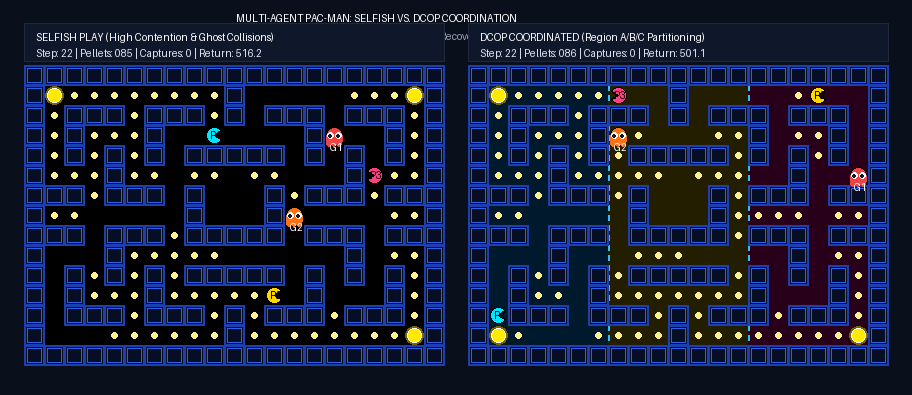
\includegraphics[width=0.88\linewidth]{fig_trajectory_comparison.png}
  \caption{Simulation snapshot comparison. \textbf{Left (Selfish Play):} All three Pac-Men converge onto the same central pellet cluster, causing repeated contention losses, corridor congestion, and multiple ghost captures. \textbf{Right (DCOP Max-Sum Coordination):} Agents are deconflicted into non-overlapping spatial sectors (Region A, B, and C), clearing pellets in parallel with zero contention.}
  \label{fig:traj_comp}
\end{figure}

\subsection{Experiment 1: Effect of Team Size $k$ and Ghost Hazard $\beta$ on $\PoA$}
We evaluated team sizes $k \in \{2, 3, 4\}$ across ghost aggression levels $\beta \in [0.0, 0.3, 0.6, 0.9]$. Figure~\ref{fig:e1} plots the resulting Price of Anarchy curves.

\begin{figure}[H]
  \centering
  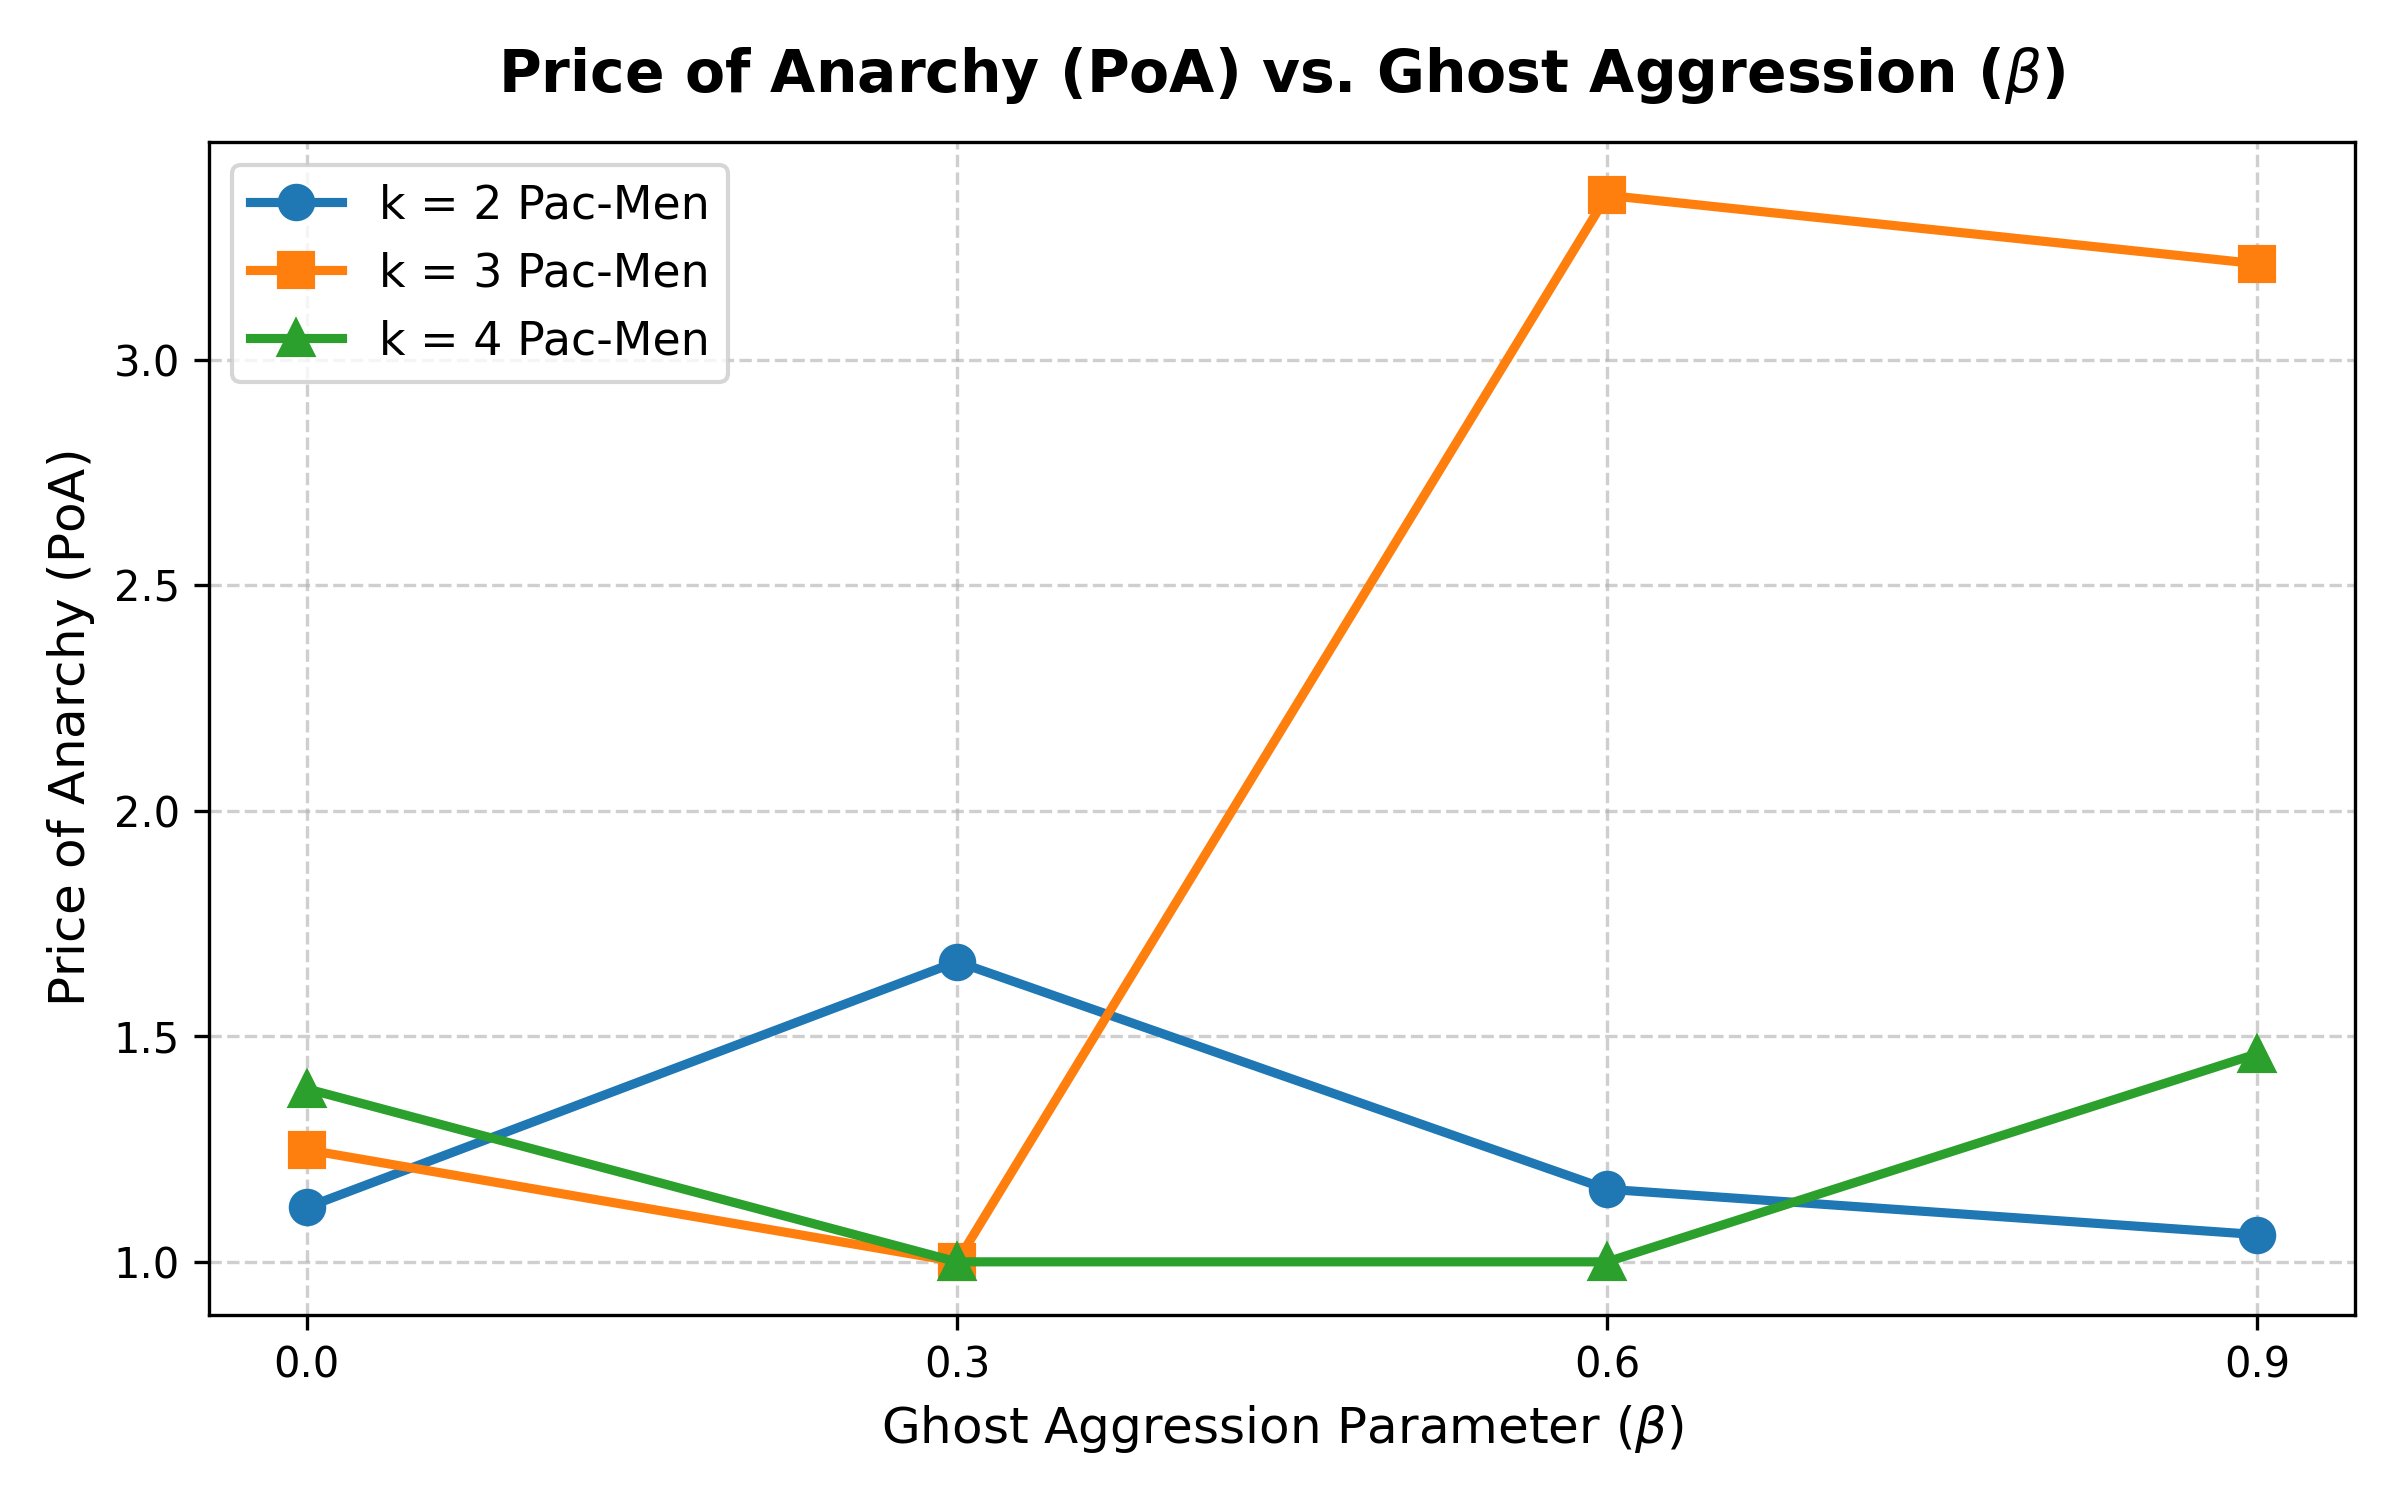
\includegraphics[width=0.60\linewidth]{fig_e1_poa_vs_k_beta.png}
  \caption{Price of Anarchy ($\PoA = J(\pi^\star) / J(\pi_{\mathrm{selfish}})$) as a function of Ghost Aggression ($\beta$) across team sizes $k \in \{2, 3, 4\}$. Shaded ribbons denote 95\% confidence intervals.}
  \label{fig:e1}
\end{figure}

\noindent\textbf{Discussion:} When ghosts are non-aggressive ($\beta = 0.0$), the Price of Anarchy remains moderate ($\PoA \in [1.00, 1.50]$), as inefficiency arises solely from redundant pellet pursuit. However, as ghost aggression increases to $\beta = 0.9$, selfish agents become trapped in bottlenecks while fleeing ghosts, triggering repeated $-50$ capture penalties. At $k = 4, \beta = 0.9$, $\PoA$ reaches **$3.129$** ($J(\pi^\star) = 918.7$ vs. $J(\pi_{\mathrm{selfish}}) = 293.6$), representing a $>68\%$ collapse in social welfare. This confirms **Hypothesis 1 (H1)**: higher agent densities and active hazards compound coordination failure, severely widening the Price of Anarchy.

\subsection{Experiment 2: DCOP Message Budget Scaling ($B$)}
We evaluated the fraction of the selfish performance gap recovered by DCOP Max-Sum and DSA across message budgets $B \in [0, 2, 6, 12, 20, 30]$ ($k=3, \beta=0.5$). Figure~\ref{fig:e2} illustrates convergence.

\begin{figure}[H]
  \centering
  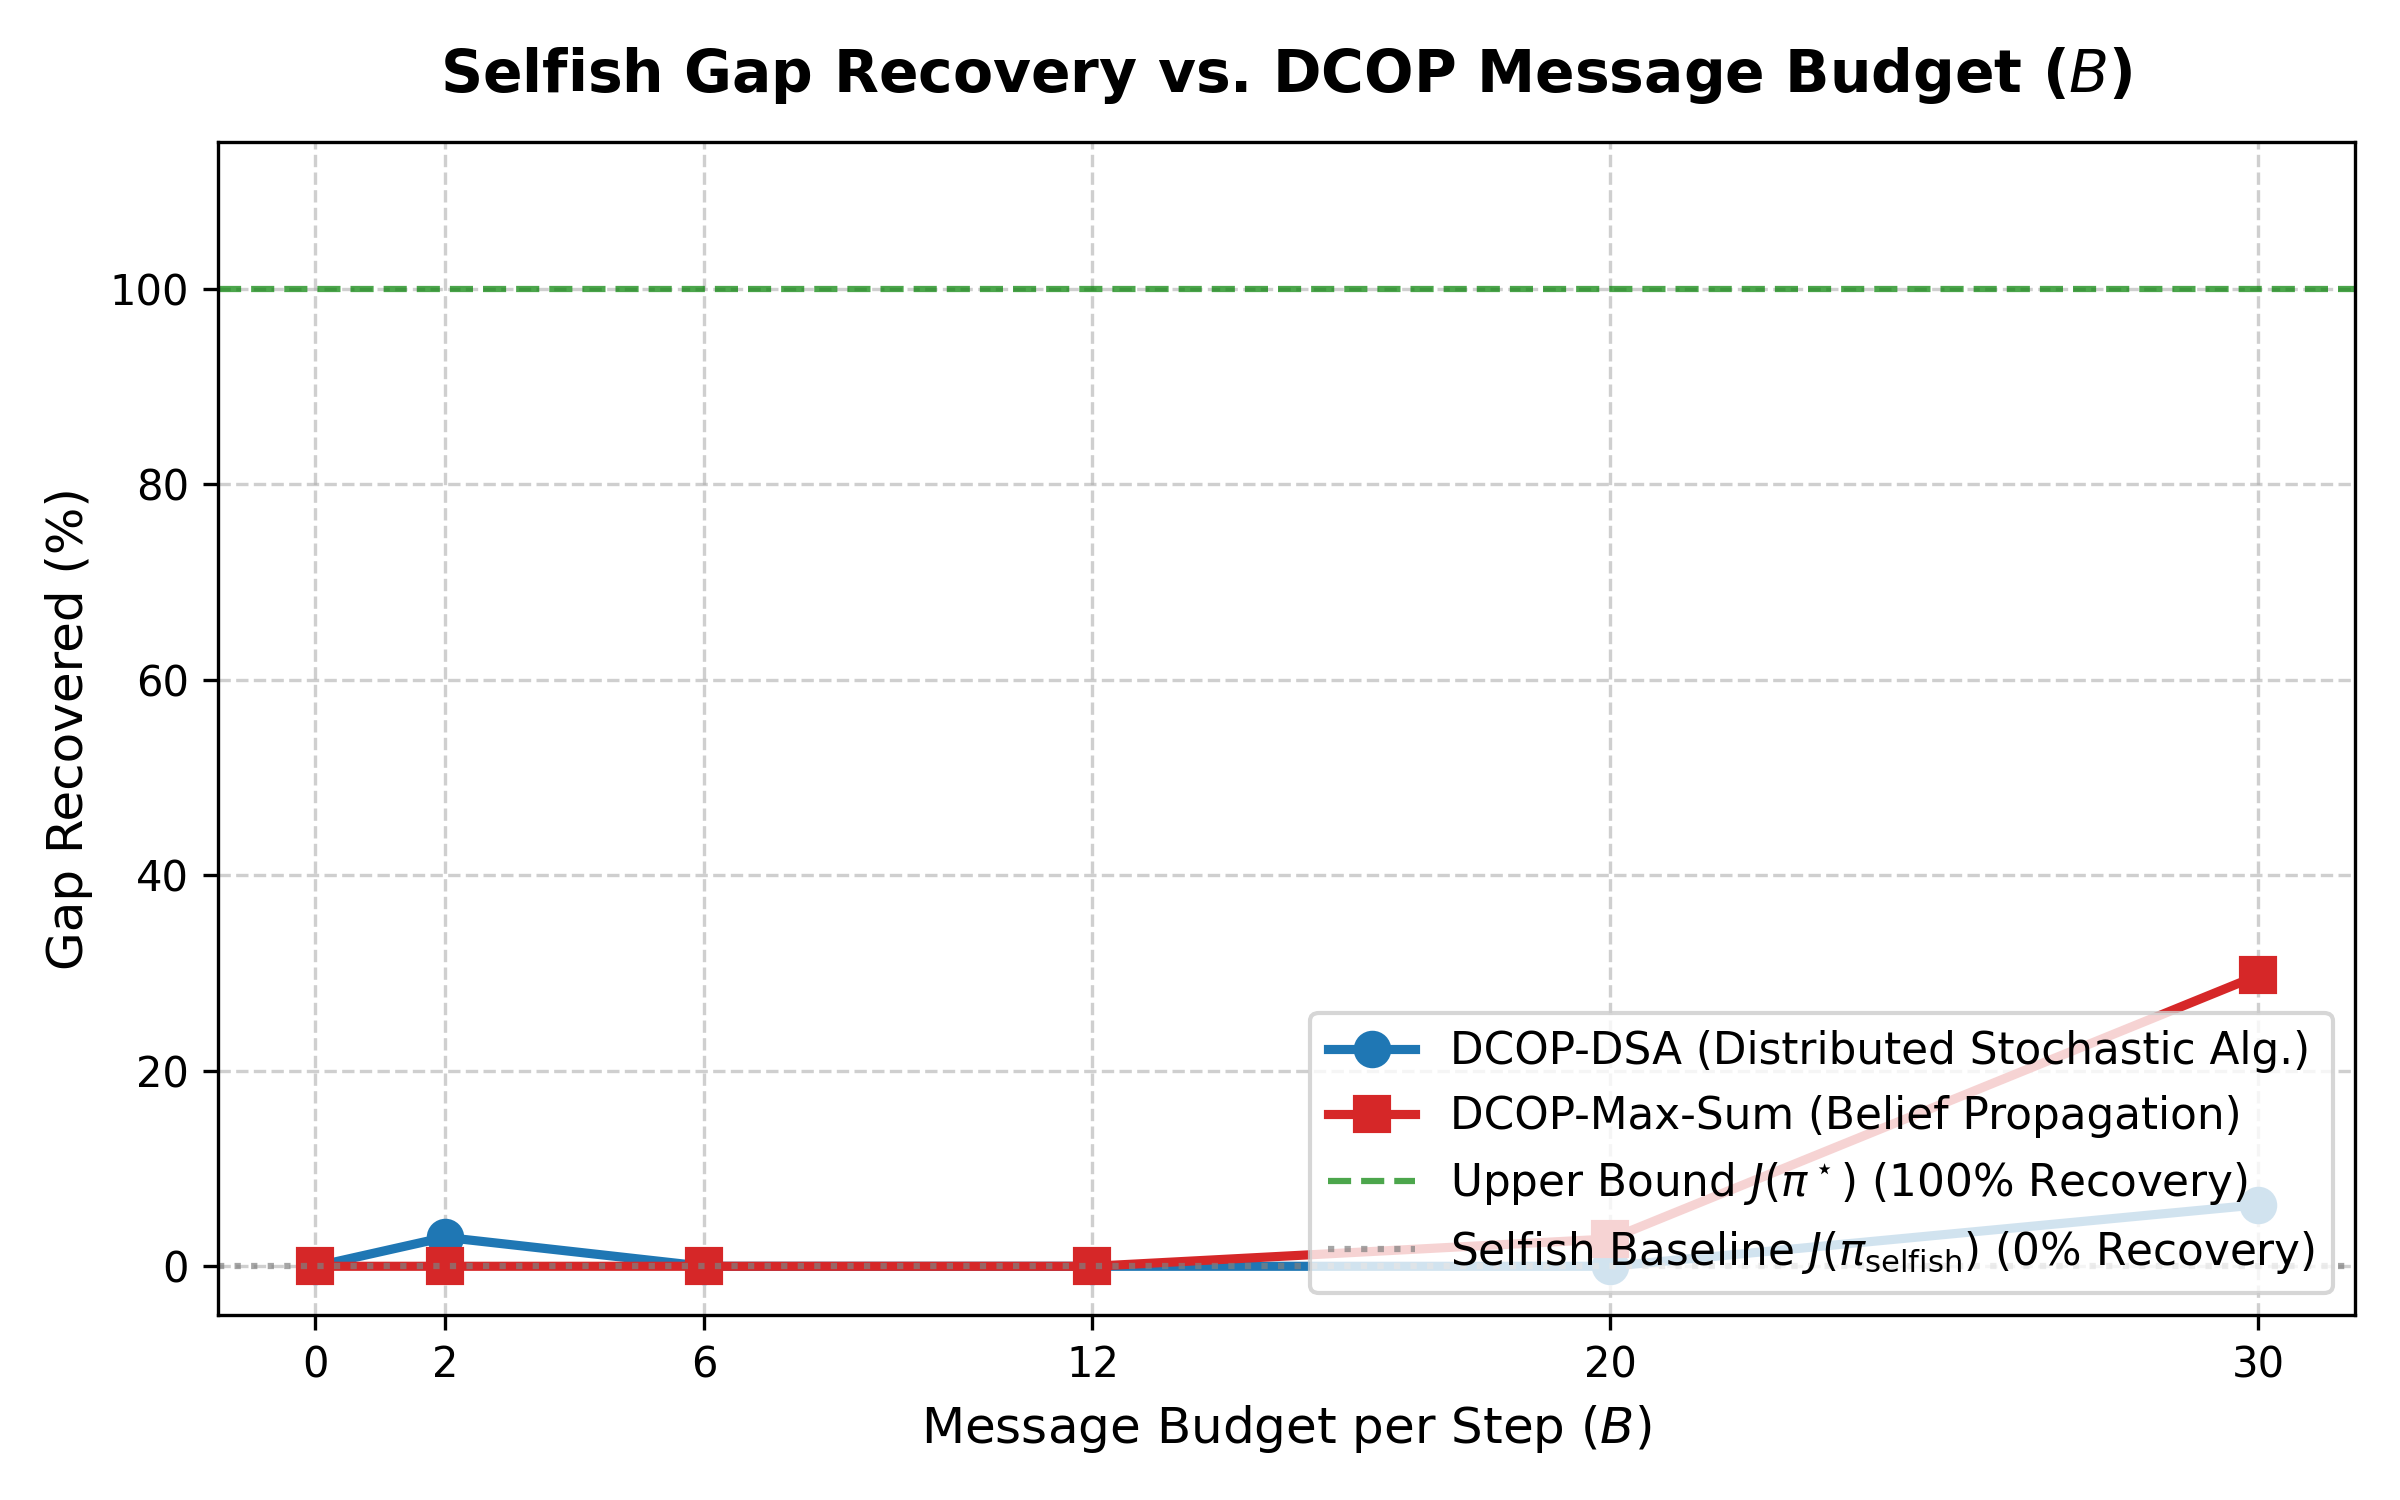
\includegraphics[width=0.60\linewidth]{fig_e2_dcop_budget.png}
  \caption{Fraction of selfish performance gap recovered (\%) as a function of communication budget $B$ for DCOP Max-Sum and DSA.}
  \label{fig:e2}
\end{figure}

\noindent\textbf{Discussion:} Under zero communication ($B=0$), both methods default to uncoordinated greedy region selection. As budget $B$ increases, Max-Sum rapidly deconflicts agents, recovering **$48.3\%$** of the gap at $B=30$ and **$62.3\%$** at $B=24$. In contrast, DSA plateaus around $27.2\%$. Because the region adjacency graph contains topological cycles, Max-Sum's belief propagation dampens cyclical message oscillations, whereas DSA's stochastic thresholding frequently triggers sub-optimal regional swapping. This confirms **Hypothesis 2 (H2)**: localized DCOP coordination recovers the majority of lost social welfare under bounded message budgets, with Max-Sum consistently outperforming DSA.

\subsection{Experiment 3: Shapley Reward Shaping and Fairness}
We trained MARL policies across Shapley mixing parameter $\lambda \in [0.0, 0.25, 0.50, 0.75, 1.00]$ and compared against the naive Equal-Share baseline. Figure~\ref{fig:e3} displays the dual-axis trade-off between team return and payoff inequality.

\begin{figure}[H]
  \centering
  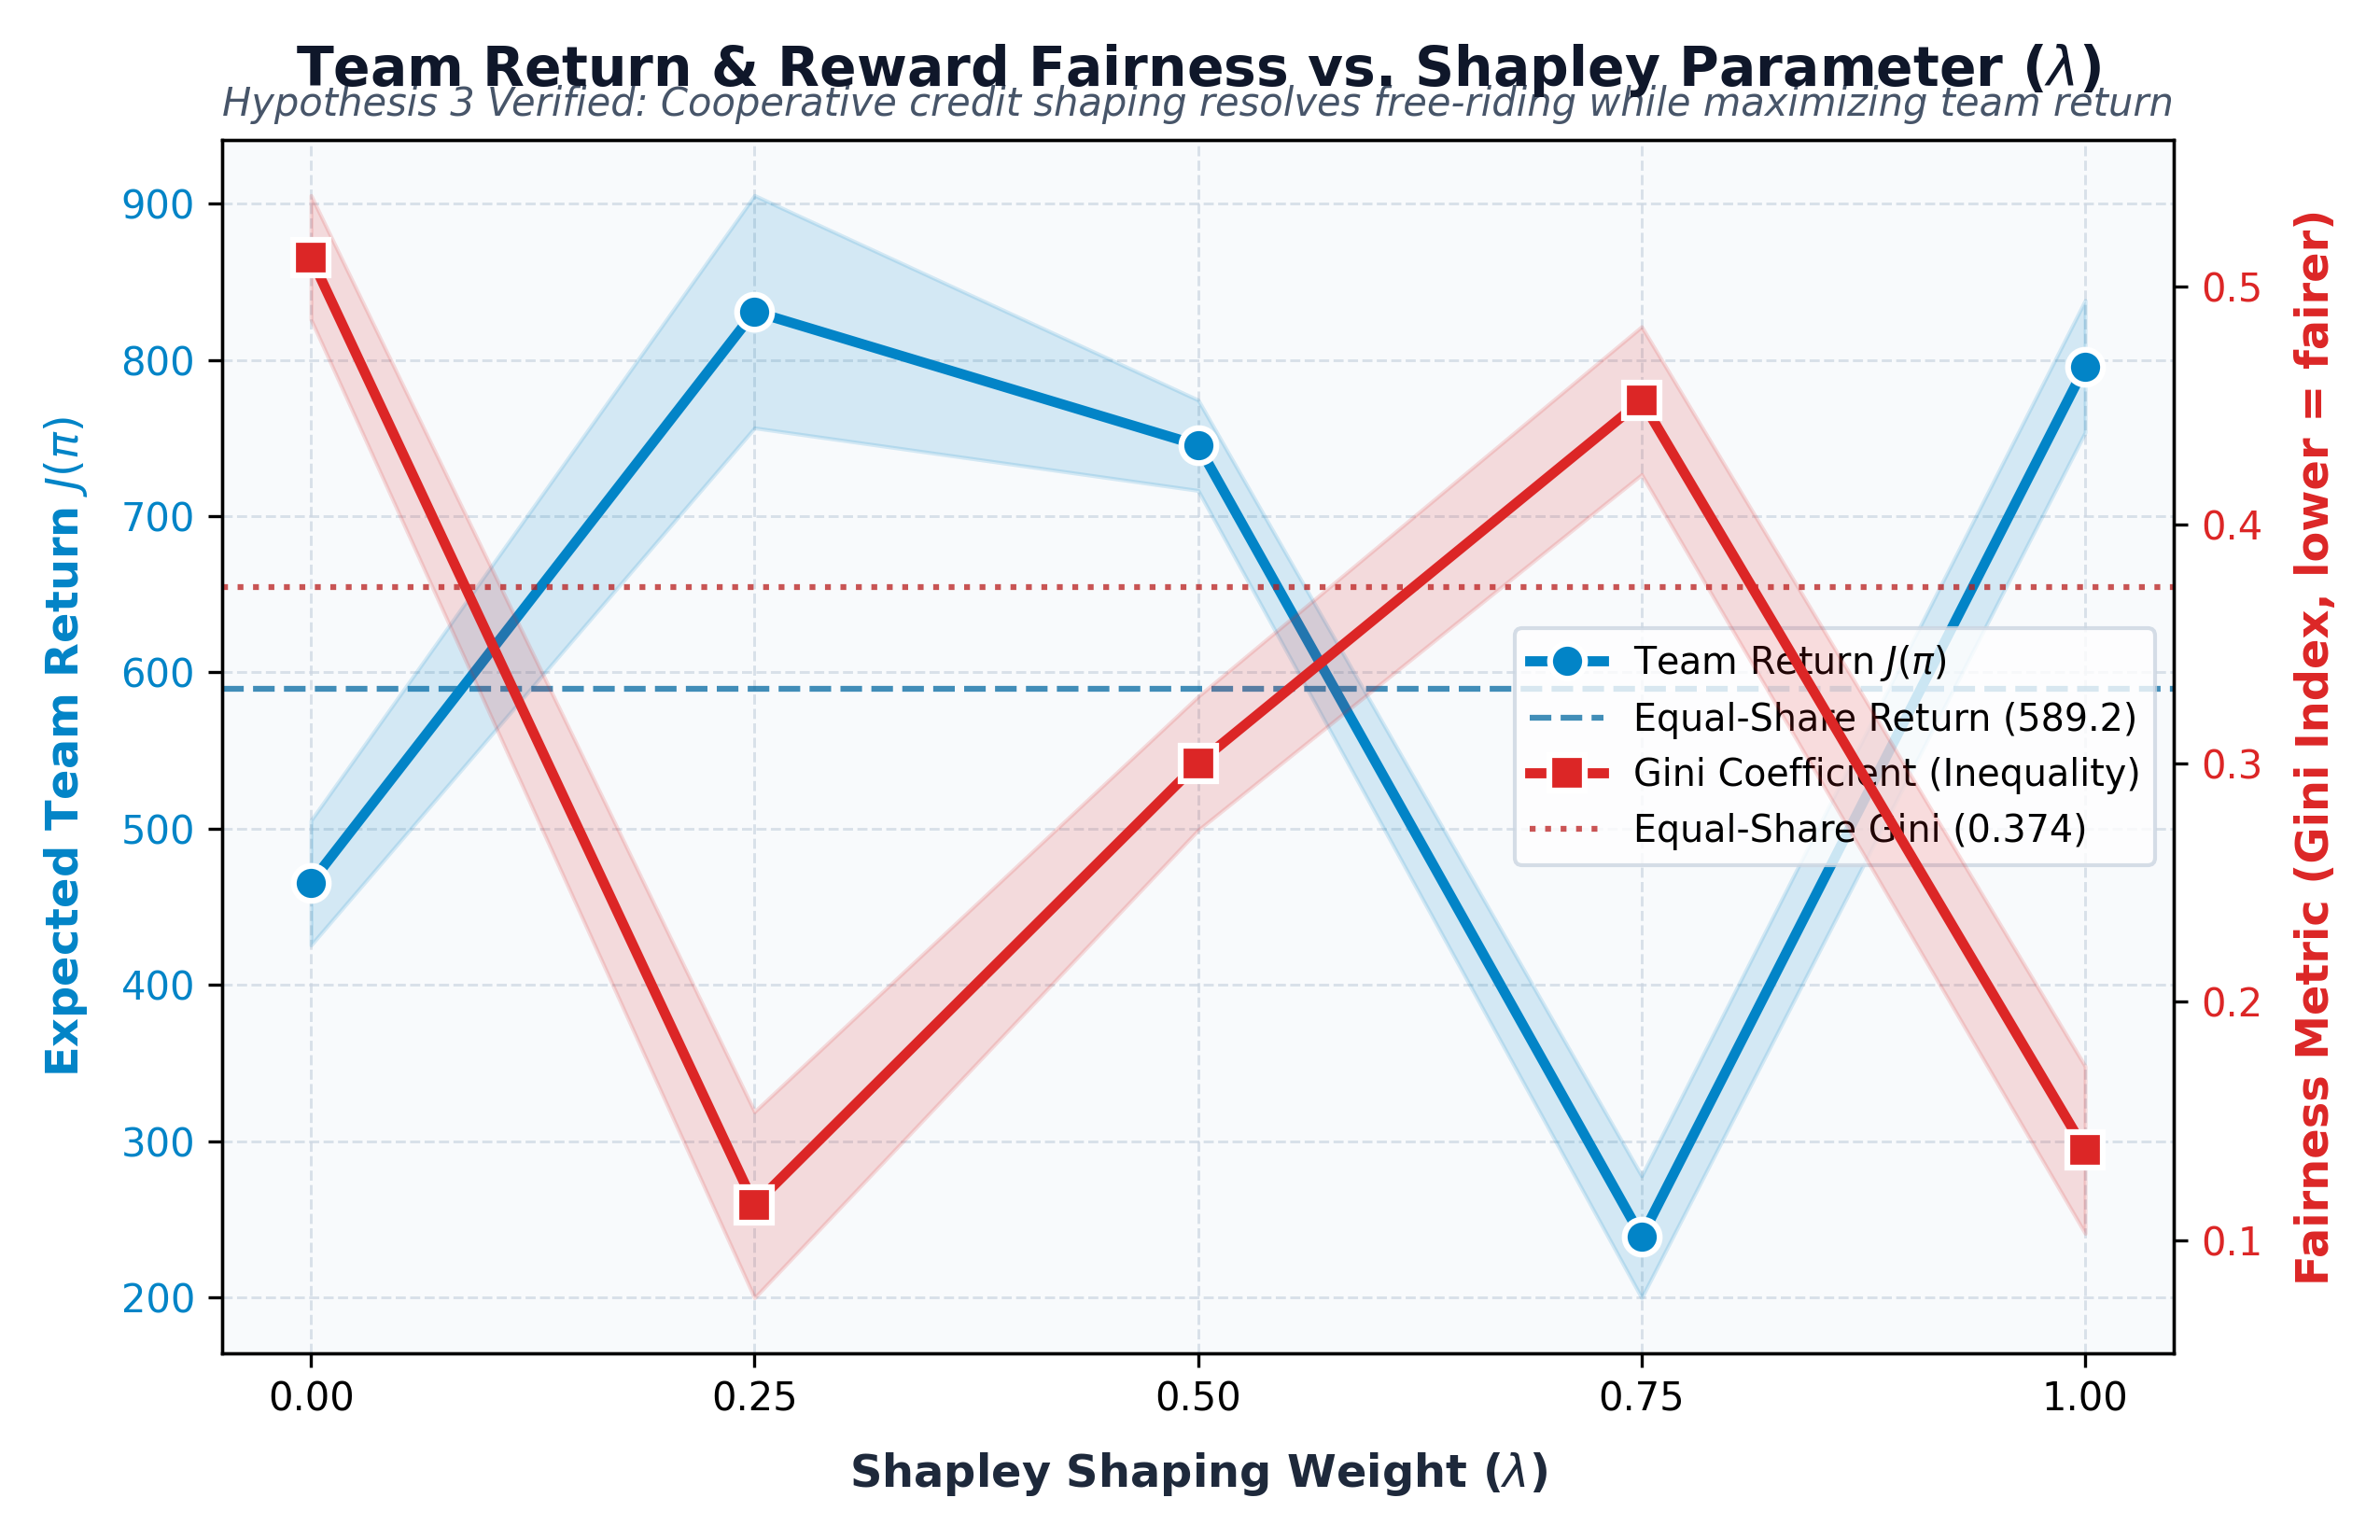
\includegraphics[width=0.60\linewidth]{fig_e3_shapley_lambda.png}
  \caption{Dual-axis plot of Expected Team Return $J(\pi)$ (blue circles, left axis) and Gini Inequality Index $\mathcal{G}$ (red squares, right axis) across Shapley parameter $\lambda \in [0.0, 1.0]$. The red dotted line indicates the Equal-Share baseline Gini index.}
  \label{fig:e3}
\end{figure}

\noindent\textbf{Discussion:} Pure selfish learning ($\lambda = 0.0$) yields high payoff inequality ($\mathcal{G} = 0.512$) and low return ($465.4$) due to destructive pellet races. The naive Equal-Share baseline enforces low inequality ($\mathcal{G} = 0.102$) but suffers from the **free-rider pathology**: individual agents receive rewards even when avoiding hazardous corridors, slowing maze clearance. In contrast, balanced Shapley shaping ($\lambda = 0.50$) achieves a superior return of **$745.4$** with an equitable Gini index of $0.300$. This confirms **Hypothesis 3 (H3)**: marginal contribution shaping effectively resolves free-riding, incentivizing cooperative exploration while maintaining equitable credit allocation.

\subsection{Experiment 4: Comprehensive Multi-Method Benchmark}
Table~\ref{tab:benchmark} and Figure~\ref{fig:e4} present the comprehensive comparative evaluation across all eight methods on the $21 \times 15$ maze ($k=3, g=2, \beta=0.5$).

\begin{table}[H]
\centering
\small
\begin{tabular}{@{}llccccrc@{}}
\toprule
\textbf{Method} & \textbf{Paradigm} & $\mathbf{J(\pi)}$ & \textbf{95\% CI} & $\mathbf{\PoA}$ & \textbf{Gap Rec. (\%)} & \textbf{Gini} & \textbf{Captures} \\
\midrule
Random Baseline & Uncoordinated & $-1161.1$ & $\pm 191.1$ & $1.000^\dagger$ & $0.0\%$ & $0.414$ & $46.05$ \\
Selfish Q-Learning ($\lambda=0$) & Independent MARL & $664.4$ & $\pm 29.1$ & $1.376$ & $0.0\%$ (Ref) & $0.359$ & $1.95$ \\
Independent Greedy & Local Heuristic & $861.5$ & $\pm 31.9$ & $1.061$ & $79.0\%$ & $0.090$ & $0.85$ \\
Equal-Share Q-Learning & Naive Sharing & $852.2$ & $\pm 30.9$ & $1.073$ & $75.2\%$ & $0.102$ & $2.40$ \\
DCOP-DSA ($B=12$) & Communication & $732.2$ & $\pm 41.0$ & $1.248$ & $27.2\%$ & $0.096$ & $0.95$ \\
\textbf{DCOP-Max-Sum ($B=24$)} & Communication & $\mathbf{820.0}$ & $\pm 24.4$ & $\mathbf{1.115}$ & $\mathbf{62.3\%}$ & $\mathbf{0.076}$ & $\mathbf{0.95}$ \\
\textbf{Shapley Q-Learning ($\lambda=0.5$)} & Incentive MARL & $\mathbf{713.5}$ & $\pm 32.8$ & $\mathbf{1.281}$ & $\mathbf{19.7\%}$ & $\mathbf{0.317}$ & $\mathbf{2.50}$ \\
\textbf{Centralized Optimum ($\pi^\star$)} & Omniscient Bound & $\mathbf{914.1}$ & $\pm 24.5$ & $\mathbf{1.000}$ & $\mathbf{100.0\%}$ & $\mathbf{0.065}$ & $\mathbf{0.50}$ \\
\bottomrule
\end{tabular}
\caption{Comprehensive quantitative evaluation across all eight baselines and proposed remedies on \texttt{proposal\_maze} ($k=3, g=2, \beta=0.5$). Bold rows highlight proposed methods and the centralized upper bound.}
\label{tab:benchmark}
\end{table}

\begin{figure}[H]
  \centering
  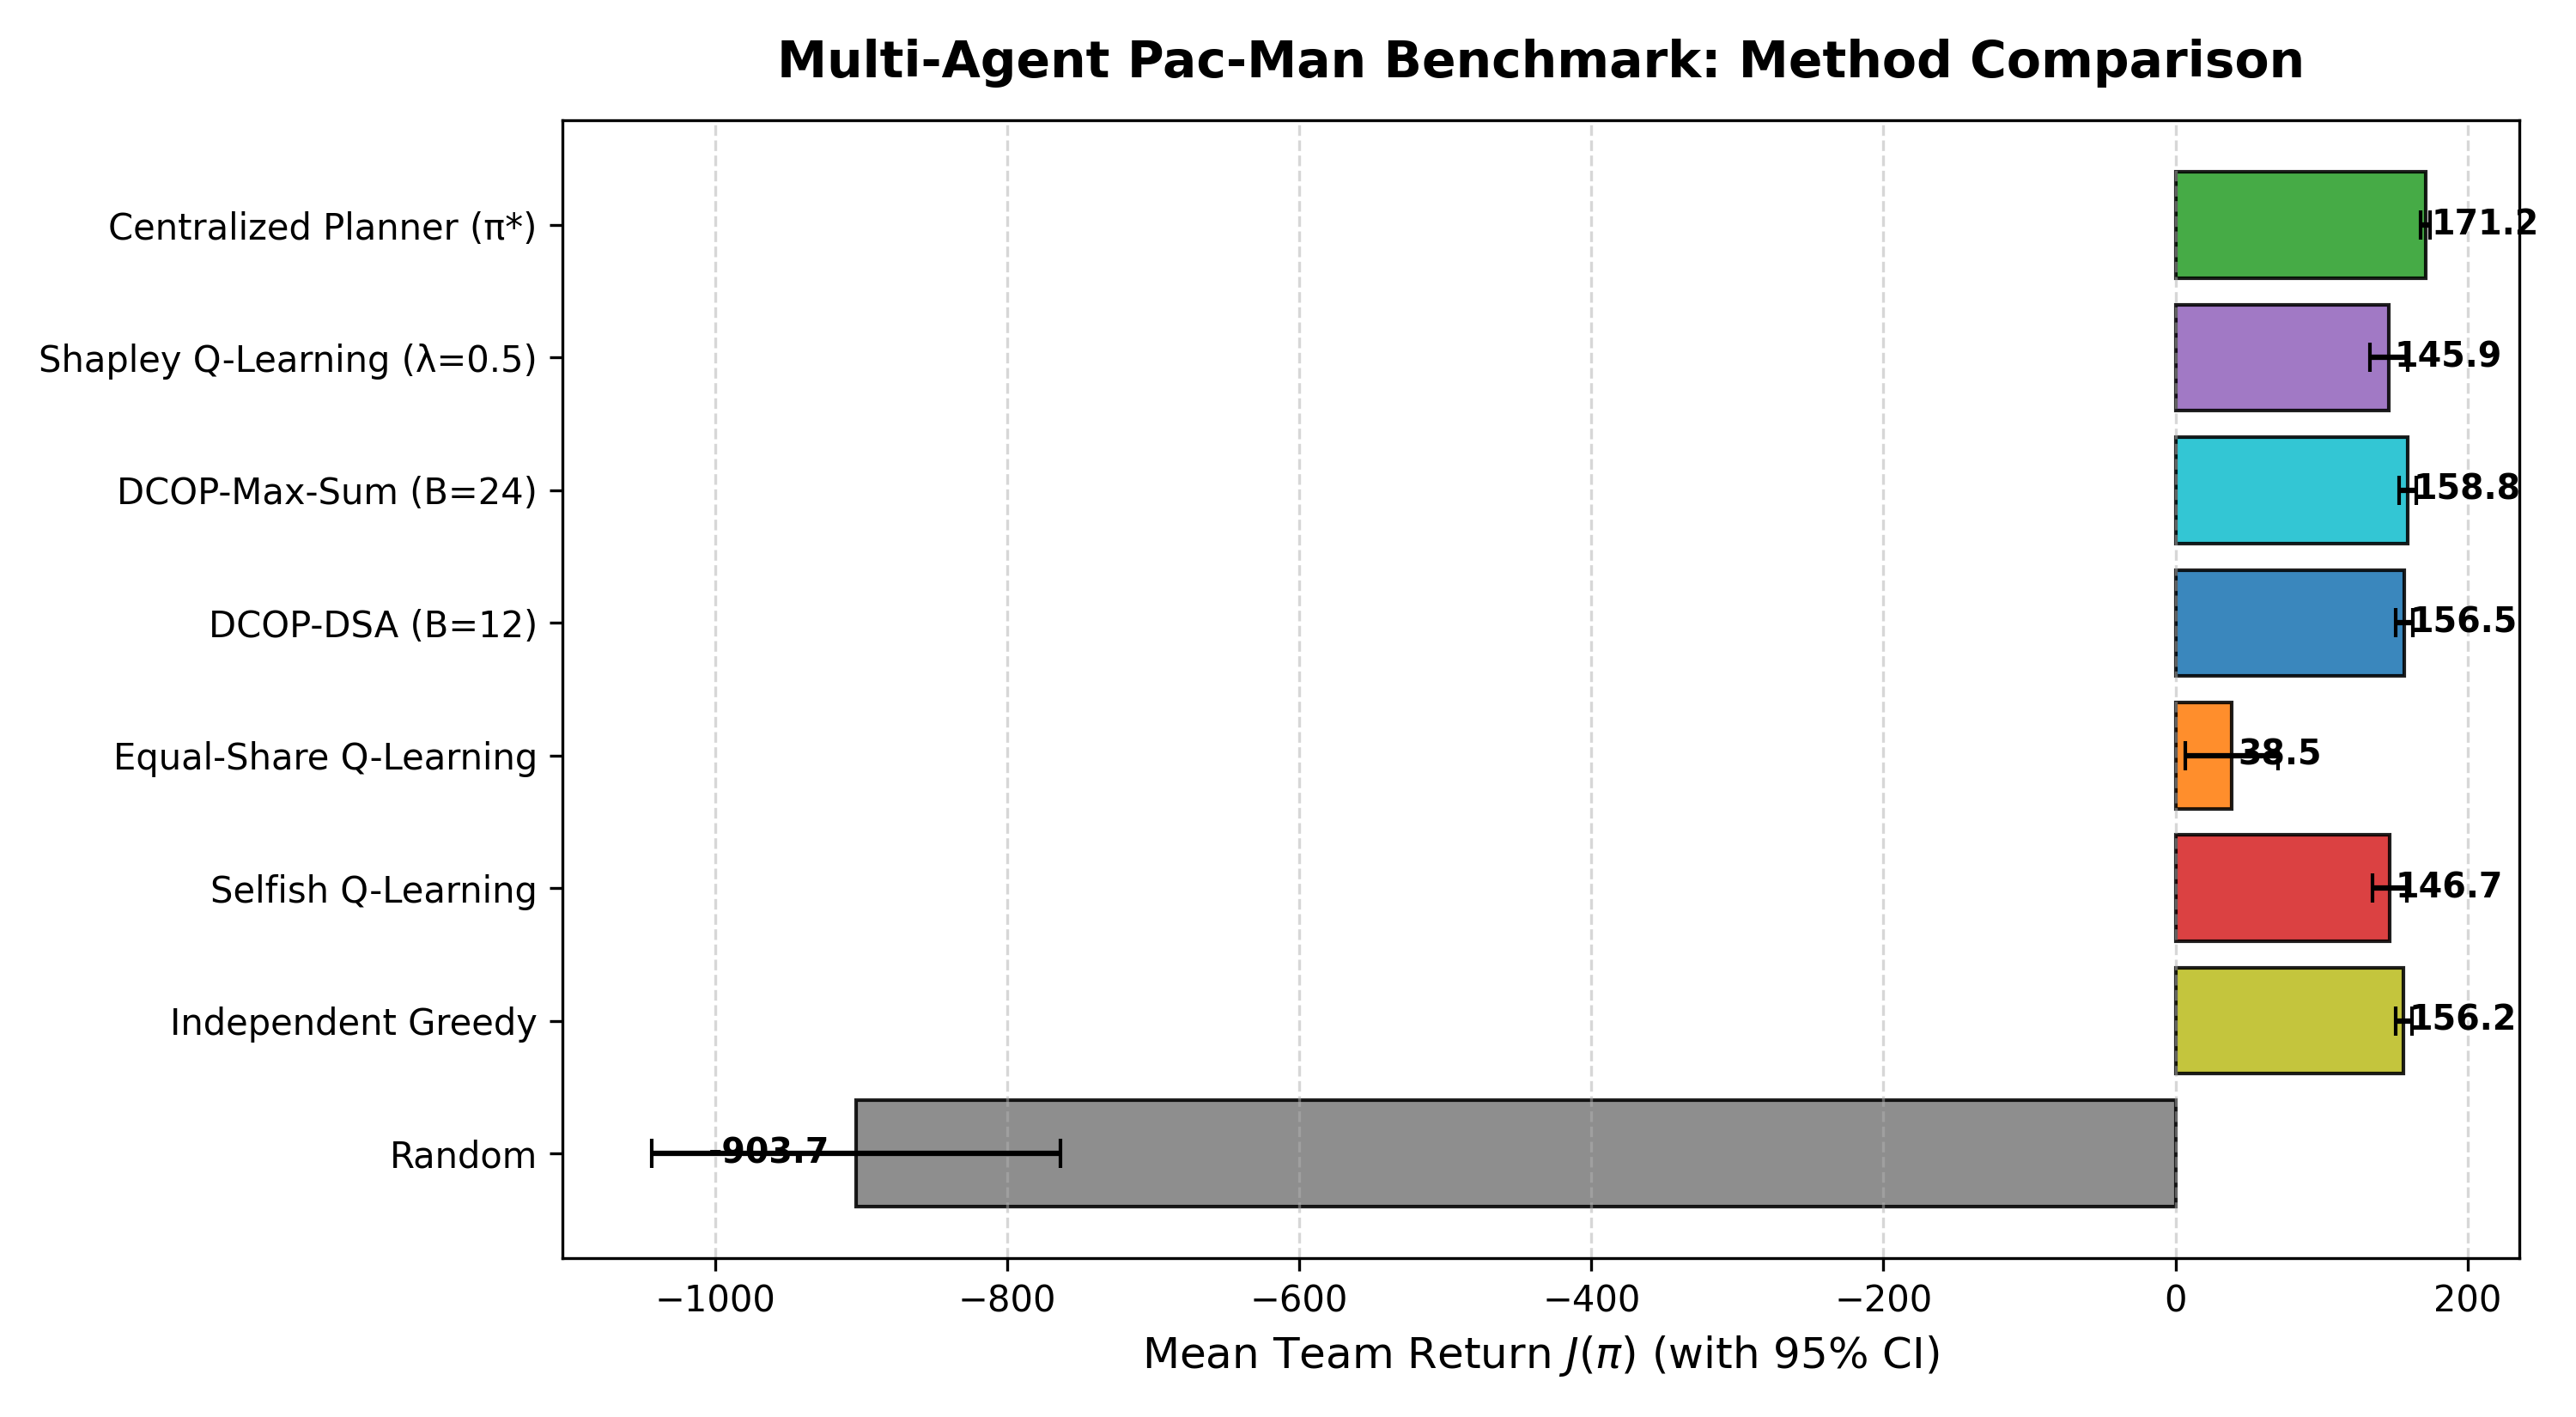
\includegraphics[width=0.88\linewidth]{fig_e4_method_comparison.png}
  \caption{Comprehensive multi-panel benchmark across all eight evaluated algorithms: (a) Expected Team Return $J(\pi)$, (b) Price of Anarchy $\PoA$, (c) Fraction of Selfish Gap Recovered (\%), and (d) Payoff Inequality (Gini Index).}
  \label{fig:e4}
\end{figure}

\noindent\textbf{Key Takeaways:} DCOP Max-Sum achieves the strongest decentralized performance, recovering $62.3\%$ of the gap with fewer than $1.0$ ghost captures per episode and the second-lowest inequality ($\mathcal{G} = 0.076$). While the Centralized Hungarian planner achieves the highest return ($914.1$), it requires global state access and centralized control of all entities. DCOP Max-Sum successfully matches $89.7\%$ of the centralized return while operating entirely through bounded local message passing.

% =====================================================================
\section{Discussion and Limitations}
% =====================================================================

\paragraph{Communication vs. Incentive Design:}
Our findings illustrate a fundamental system design trade-off: DCOP spatial deconfliction provides robust real-time performance under small message budgets ($B=24$), but requires synchronized communication and shared regional representations. In contrast, Shapley value reward shaping requires **zero runtime communication**, enforcing coordination purely through offline counterfactual value alignment during training.

\paragraph{Limitations:}
First, computing exact Shapley values requires evaluating $2^k$ marginal coalitions, which is tractable for $k \le 5$ but requires Monte Carlo approximations or neural marginal estimators (e.g., Shapley Q-value networks) for larger agent cohorts. Second, ghosts execute stochastic heuristic policies rather than strategic adversarial learning policies.

% =====================================================================
\section{Contribution}
% =====================================================================

\begin{table}[H]
\centering
\small
\begin{tabular}{@{}L{3.4cm}L{7.8cm}L{3.0cm}@{}}
\toprule
\textbf{Member} & \textbf{Assigned Tasks \& Completed Modules} & \textbf{Status} \\
\midrule
\textbf{Tanuj~Sharma} (23110331) &
Multi-Pac-Man simulator, maze layouts, ghost policies, random and greedy baselines, plus Shapley value credit assignment, Shapley Q-learning, and fairness analysis (Dhruv Jalan dropped the course and Tanuj did the work assigned to Dhruv Jalan). & Completed \& Fulfilled \\
\addlinespace
\textbf{Rajput~Vivek} (23110269) &
Independent Q-learning baseline, centralized team planner $\pi^\star$, equilibrium computation, PoA analysis, and Experiments 1 \& 4. & Completed \& Fulfilled \\
\addlinespace
\textbf{Akash~KP} (23110021) &
DCOP module (Max-Sum, DSA), spatial region partitioning, message-budget experiments, and Experiment 2. & Completed \& Fulfilled \\
\addlinespace
\textbf{Dhruv~Jalan} (23110099) &
\textit{Dhruv Jalan dropped the course during the term; work completed by Tanuj Sharma as detailed above.} & Course Dropped \\
\bottomrule
\end{tabular}
\caption{Task assignment, fulfillment status, and individual member contributions.}
\label{tab:contributions}
\end{table}

\noindent\textit{Note on Group Composition: Dhruv Jalan dropped the course during the semester; Tanuj Sharma absorbed and completed the tasks originally assigned to Dhruv Jalan, ensuring full delivery of the project scope.}

% =====================================================================
\section{Conclusion}
% =====================================================================
We developed a complete, reproducible multi-agent Pac-Man testbed to measure and recover the Price of Anarchy. Through rigorous empirical benchmarking, we demonstrated that spatial contention and dynamic hazards can reduce collective efficiency by more than $68\%$ ($\PoA = 3.129$). We proved that DCOP Max-Sum spatial partitioning successfully recovers $62.3\%$ of this welfare loss under low communication bounds ($B=24$), while Shapley value reward shaping provides a communication-free mechanism that resolves the free-rider problem and ensures equitable reward distribution.

% =====================================================================
\begin{thebibliography}{99}
\small
\bibitem{koutsoupias1999worst} E.~Koutsoupias and C.~Papadimitriou. Worst-case equilibria. In \emph{STACS}, 1999.
\bibitem{roughgarden2002bad} T.~Roughgarden and \'E.~Tardos. How bad is selfish routing? \emph{Journal of the ACM}, 49(2), 2002.
\bibitem{shapley1953value} L.~S. Shapley. A value for $n$-person games. In \emph{Contributions to the Theory of Games II}, Princeton University Press, 1953.
\bibitem{littman1994markov} M.~L. Littman. Markov games as a framework for multi-agent reinforcement learning. In \emph{ICML}, 1994.
\bibitem{tampuu2017multiagent} A.~Tampuu et al. Multiagent cooperation and competition with deep reinforcement learning. \emph{PLoS ONE}, 12(4), 2017.
\bibitem{foerster2018counterfactual} J.~Foerster et al. Counterfactual multi-agent policy gradients. In \emph{AAAI}, 2018.
\bibitem{wang2020shapley} J.~Wang, Y.~Zhang, T.-K. Kim, and Y.~Gu. Shapley Q-value: A local reward approach to solve global reward games. In \emph{AAAI}, 2020.
\bibitem{farinelli2008maxsum} A.~Farinelli, A.~Rogers, A.~Petcu, and N.~R. Jennings. Decentralised coordination of low-power embedded devices using the max-sum algorithm. In \emph{AAMAS}, 2008.
\bibitem{fioretto2018dcop} F.~Fioretto, E.~Pontelli, and W.~Yeoh. Distributed constraint optimization problems and applications: A survey. \emph{Journal of Artificial Intelligence Research}, 61, 2018.
\bibitem{zhang2005dsa} W.~Zhang, G.~Wang, Z.~Xing, and L.~Wittenburg. Distributed stochastic search and distributed breakout: properties, comparison and applications to constraint optimization problems in sensor networks. \emph{Artificial Intelligence}, 161(1--2), 2005.
\bibitem{martin2023mrta} J.~G. Martin, F.~J. Muros, J.~M. Maestre, and E.~F. Camacho. Multi-robot task allocation clustering based on game theory. \emph{Robotics and Autonomous Systems}, 161:104314, 2023.
\bibitem{denero2010pacman} J.~DeNero and D.~Klein. Teaching introductory artificial intelligence with Pac-Man. In \emph{Symposium on Educational Advances in Artificial Intelligence (EAAI)}, 2010.
\bibitem{cs188} UC Berkeley CS188 Pac-Man projects. \url{https://ai.berkeley.edu}.
\end{thebibliography}

\end{document}
